%\documentclass[serif,mathserif,notes]{beamer}
\documentclass[serif,mathserif,notes=hide]{beamer}
%\documentclass[serif,mathserif,notes=only]{beamer}
\usepackage[portuguese]{babel}
\usepackage[utf8]{inputenc}
\usepackage{amsmath, amsfonts, epsfig, xspace}
\usepackage{algorithm,algorithmic}
\usepackage{pstricks,pst-node}
\usepackage{multimedia}
\usepackage[normal,tight,center]{subfigure}
\setlength{\subfigcapskip}{-.5em}
\usepackage[font=scriptsize]{caption} %Diminuindo tamanho da caption
\usepackage{beamerthemesplit}
\usetheme{lankton-keynote}
\setbeamerfont{title}{size=\large}
%\setbeameroption{show only notes}
%\setbeameroption{hide notes}
\setbeamercolor{note page}{bg=white!90!black, fg=black}
\setbeamercolor{note title}{bg=white!80!black, fg=black}
\setbeamercolor{note date}{parent=note title}


\newcommand{\CcImageBy}[1]{%
  
\includegraphics[scale=#1]{src/img/creative_commons/cc_by_30.pdf}%
}
\newcommand{\CcImageSa}[1]{%
  
\includegraphics[scale=#1]{src/img/creative_commons/cc_sa_30.pdf}%
}
\newcommand{\CcGroupBySa}[2]{% zoom, gap
  \CcImageBy{#1}\hspace*{#2}\CcImageSa{#1}%
}
\newcommand{\CcLongnameBySa}{Attribution-ShareAlike}
\newcommand{\CcNote}[1]{% longname
  This work is licensed under the \textit{Creative Commons #1 3.0 License}.%
}

\author[Alessandro Palmeira\\ \and Itai Soares]{Alessandro Palmeira\\ \and Itai Soares}

\title[Instituto de Matemática e Estatística - USP\hspace{2em}\insertframenumber/\inserttotalframenumber]{Acompanhamento musical em tempo real utilizando múltiplas performances como referência}

\date{22 de Setembro de 2016} %leave out for today's date to be insterted

\institute{MAC6917 Topics in Sound and Music Computing: Music Information Retrieval}


\begin{document}


\begin{frame}
  \titlepage
  \begin{center}
    \CcGroupBySa{0.83}{0.95ex}\\
    {\tiny\CcNote{\CcLongnameBySa}}
  \end{center}
\end{frame}

\section{Apresentação}
\documentclass[xcolor=svgnames,handout]{beamer}

\usepackage[utf8x]    {inputenc}
\usepackage[T1]      {fontenc}
\usepackage[english] {babel}

\usepackage{multicol} % Pra colocar o TOC em duas colunas

\usepackage{amsmath,amsfonts,graphicx}
\usepackage{beamerleanprogress}

%------------------------------------------------
\usepackage{lmodern} % Default font: latin modern font
%\usepackage{fourier} % Alternative font: utopia
%\usepackage{charter} % Alternative font: low-resolution roman font
\usepackage{tikz} % Required for colored boxes
\usepackage{booktabs} % Required for horizontal rules in tables
\usepackage{multicol} % Required for creating multiple columns in slides
\usepackage{microtype} % Better typography
%------------------------------------------------

%------------------------------------------------
%\usetocstyle{nodotnopagenumber}

%\AtBeginDocument{\renewcaptionname{english}{\contentsname}{\Large Fases}} % Change the name of the table of contents
%------------------------------------------------

%------------------------------------------------

%----------------------------------------------------------------------------------------
%	PRESENTATION INFORMATION
%----------------------------------------------------------------------------------------
\title
  [SNES\hspace{2em}]
  {Organização de Vídeo Games\\SNES}

\author
  [Alessandro Palmeira, João M. M. da Silva]
  {Alessandro Palmeira \space\space\space\space\space\space\space\space\space\space 6850476 \\João Marco Maciel da Silva \space 7577598}

\date
  {\today}

\institute
  {Organização de Computadores - MAC0412\\Instituto de Matemática e Estatística}

%----------------------------------------------------------------------------------------
%\makeatletter
%\newtocstyle[noonewithdot]{nodotnopagenumber}{\settocfeature{pagenumberbox}{\@gobble}}
%\makeatother
%\usetocstyle{nodotnopagenumber}

%\AtBeginDocument{\renewcaptionname{english}{\contentsname}{\Large Fases}} % Change the name of the table of contents

\begin{document}
\maketitle
%	TABLE OF CONTENTS
%----------------------------------------------------------------------------------------


\begin{frame}{Índice}
\begin{multicols}{2}
  \tableofcontents
  \end{multicols}

\end{frame}

%----------------------------------------------------------------------------------------
%	PRESENTATION SLIDES
%----------------------------------------------------------------------------------------



%------------------------------------------------

\begin{frame}{História dos Vídeo Games}
\section{Visão Geral}
\subsection{História dos Vídeo Games}
\begin{itemize}
	\item Primórdios
	\begin{itemize}
		\item 1958 - "Tennis For Two".\pause
		\begin{figure}[t]
		    \centering
		    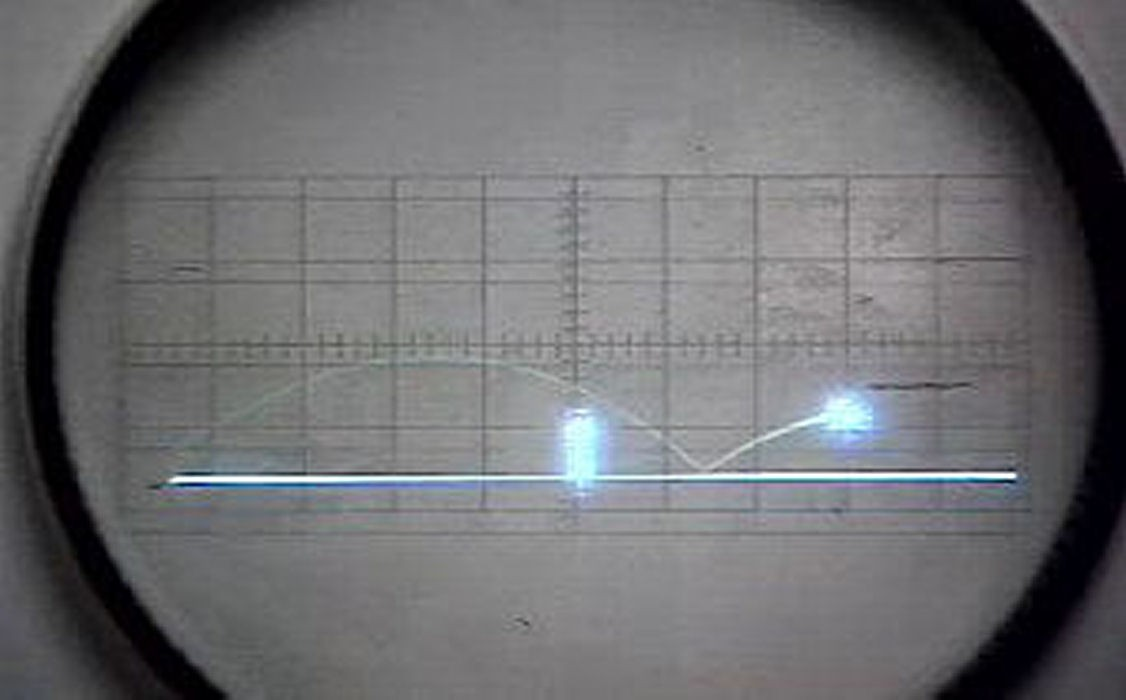
\includegraphics[scale=0.07]{imagens/tennis-for-two}
		  \end{figure}\pause
		\item 1962 - primeiro jogo em computadores dotados de transistores - "SpaceWar!"\pause
				\begin{figure}[t]
				    \centering
				    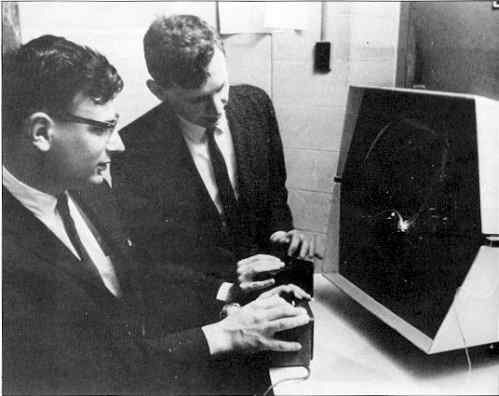
\includegraphics[scale=0.2]{imagens/golden_age3}
				  \end{figure}\pause
	\end{itemize}
\end{itemize}

\end{frame}

\begin{frame}{História dos Vídeo Games}
\begin{itemize}
	\item Primeira Geração(1972 - 1977)
	\begin{itemize}
	\item 1971 - Galaxy Game and Computer Space\pause
	\item 1972 - Odyssey 100 - primeiro vídeo game doméstico\pause
	\item 1972 - Fundação da Atari - Pong\pause
	\item 1976 - Fairchild Channel F - primeiro video game programável\pause
	\item 1977 - GunFight - primeiro jogo a usar microprocessadores\pause
	\item 1977 - crise dos Vídeo Games, só sobrevivem no mercado Atari e Magnavox\pause
	\end{itemize}
	\begin{figure}[t]
    \centering
	    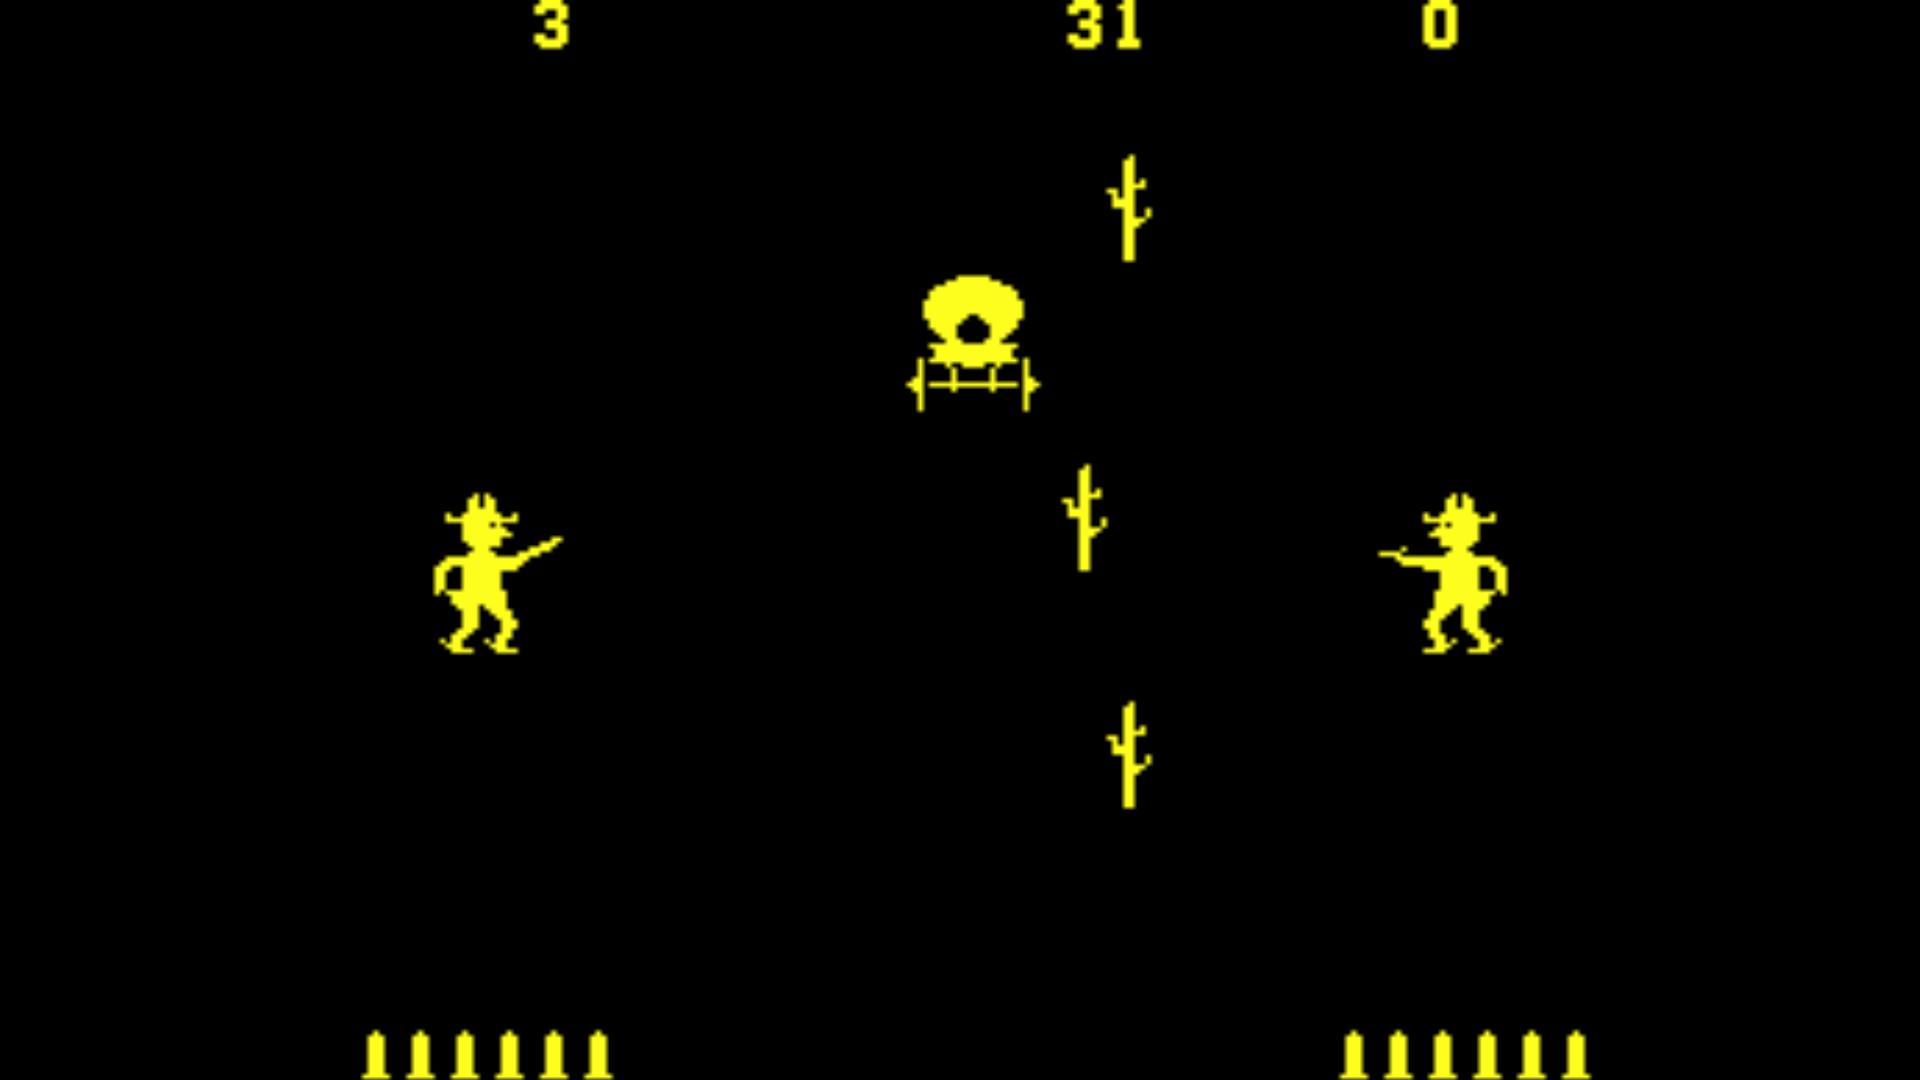
\includegraphics[scale=0.1]{imagens/gunfight}
	\end{figure}
\end{itemize}
\end{frame}
%------------------------------------------------

\begin{frame}{História dos Vídeo Games}
\begin{itemize}
	\item Segunda Geração(1977 - 1983)\pause
	\begin{itemize}
	\item 1977 - Atari 2600 - primeiro grande sucesso de vendas de consoles domésticos\pause
	\item 1978 - Nintendo entra no mercado de games\pause
	\item 1978 - Space Invaders para arcade provoca falta de moedas no mercado japonês\pause
	\item 1979 - Lunar Lander, primeiro jogo comercial com gráficos vetoriais.\pause
	\item 1979 - Sega entra para o mercado de vídeo games\pause
	\item 1980 - Pac-man\pause
	\item 1981 - Donkey Kong e Jumpman (Mario)\pause
	\item 1981 - Primeira pessoa a morrer jogando vídeo game(e não era chinês)\pause
	\item 1981 - Jogos Arcade rendem US\$5Bi\pause
	\item 1983 e 1984 - Segunda crise dos Vídeo Games
	\end{itemize}
		\begin{figure}[t]
	    \centering
		    
\includegraphics[scale=0.1]{imagens/mario}
		\end{figure}
\end{itemize}
\end{frame}

\begin{frame}{História dos Vídeo Games}
\begin{itemize}
	\item Terceira Geração(1983 - 1995)(8-bit)\pause
	\begin{itemize}
	\item 1984 - Nintendo lança o Famicom, primeiro vídeo game de sucesso com gamepad\pause
	\item 1985 - port do Super Mario Bros para Famicom\pause
	\item 1986 - Nintendo lança o Famicom nos EUA com o nome "NES"\pause
	\item 1986 - Master-System\pause
	\item 1986 - Vampire Killer(Precursor de Castlevania), The Legend of Zelda e Dragon Quest\pause
	\item 1987 - Final Fantasy e Metal Gear\pause
	\item 1988 - Fighting Street e Tetris\pause
	\item 1989 - Atari "desbloqueia" NES e lança jogos não autorizados
	\end{itemize}
		\begin{figure}[t]
	    \centering
		    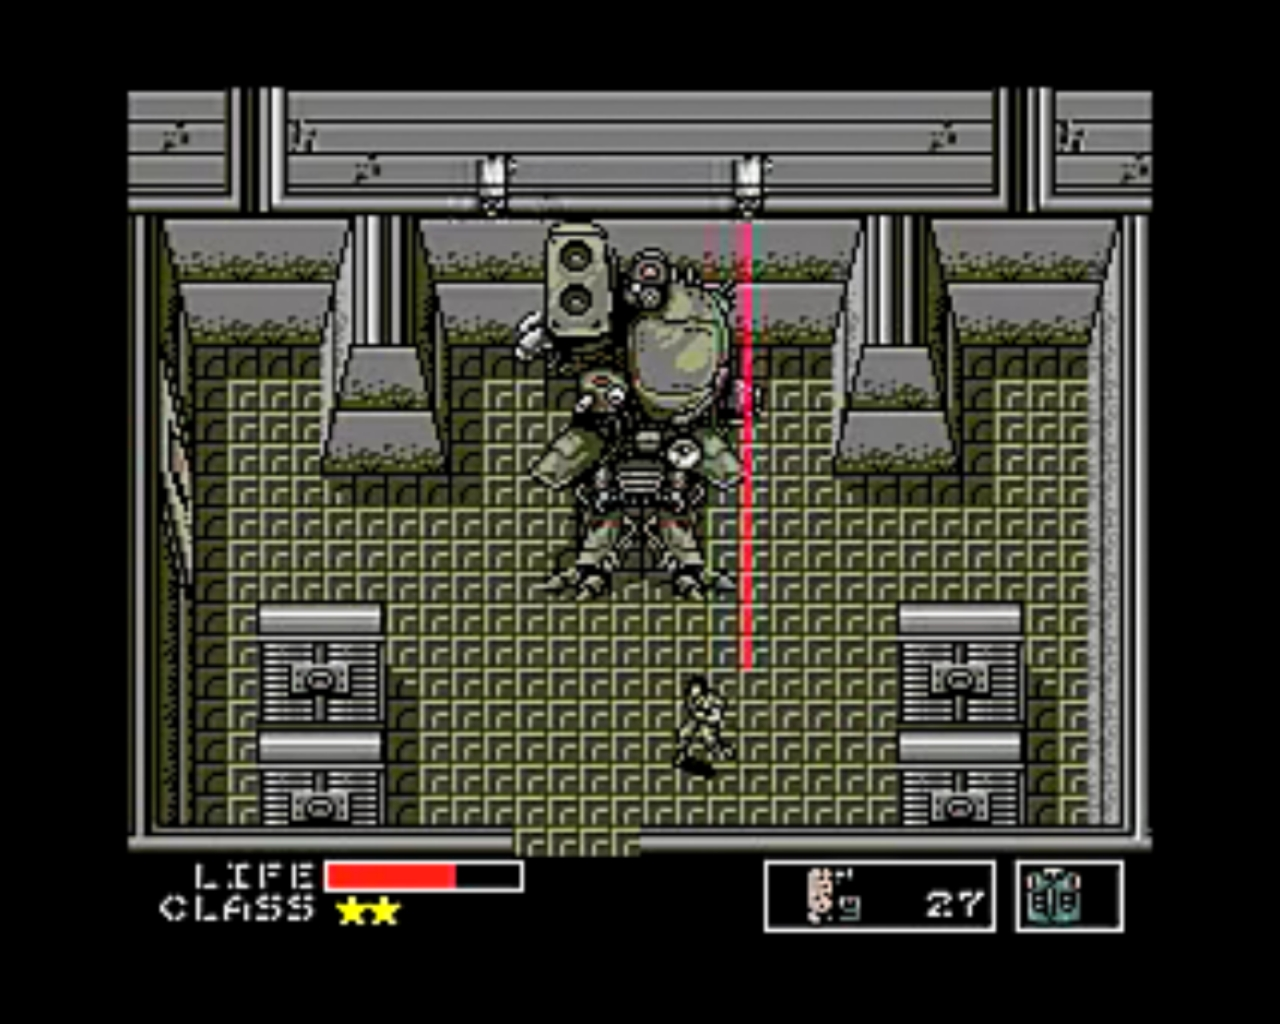
\includegraphics[scale=0.1]{imagens/metal-gear}
		\end{figure}
\end{itemize}
\end{frame}

\begin{frame}{História dos Vídeo Games}
\begin{itemize}
	\item Quarta Geração(1988 - 1999)(16-bit)\pause
	\begin{itemize}
	\item 1988 - Mega Drive/Genesis\pause
	\item 1990 - Super NES\pause
	\item 1992 - 3D básico por processadores adicionais inclusos nos cartuchos com resolução baixa e framerate < 4fps\pause
	
	\end{itemize}
		\end{itemize}
		\begin{figure}[t]
	    \centering
		    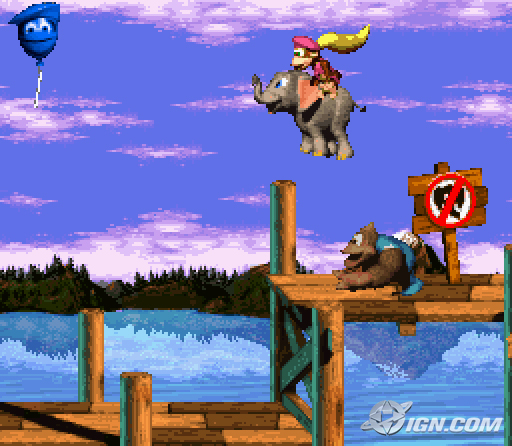
\includegraphics[scale=0.3]{imagens/dk3}
		\end{figure}
	\end{frame}
	
	\begin{frame}{História dos Vídeo Games}
		\begin{itemize}
	\item Quinta Geração(1993 - 2006)(32 e 64-bit)\pause
	\begin{itemize}
		\item Gráficos 3D, alguns Vídeo Games a CD\pause
		\item 1993 - Atari Jaguar\pause
		\item 1994 - Sega Saturn, Sony Playstation\pause
		\item 1996 - Nintendo 64\pause
		\item 1997 - Nokia lança Snake para seus celulares\pause
		\item 1998 - GameBoy\pause
		\item 2000 - China bane Vídeo Games do país\pause
		\end{itemize}
				\begin{figure}[t]
			    \centering
				    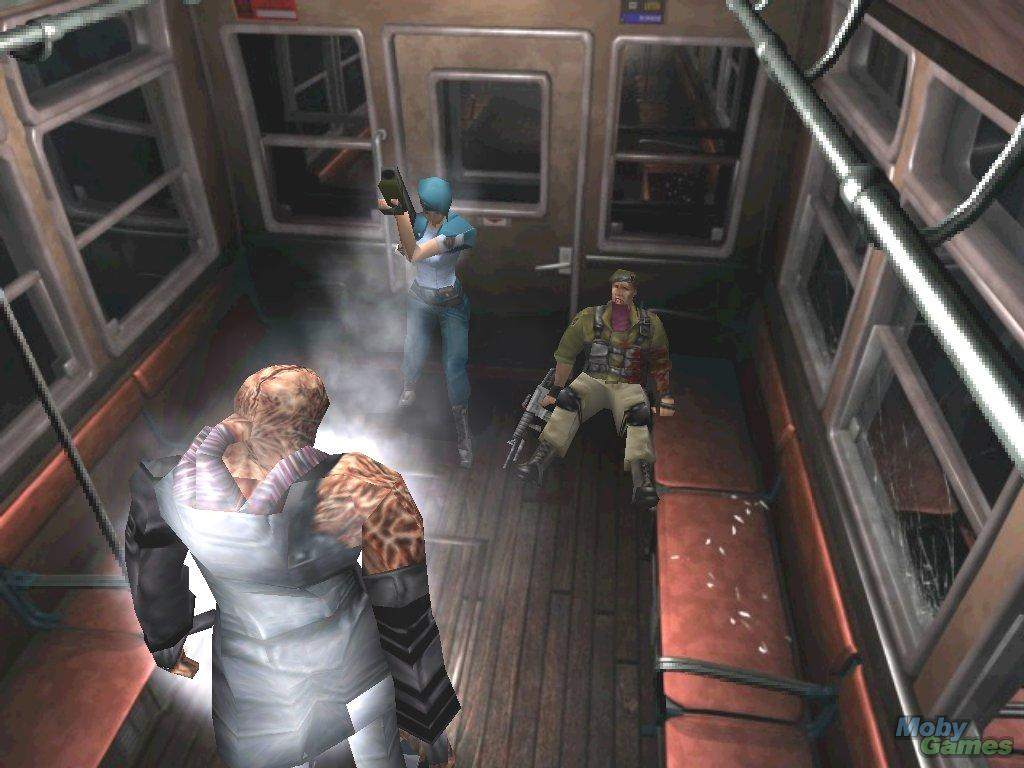
\includegraphics[scale=0.15]{imagens/re3}
				\end{figure}
\end{itemize}
\end{frame}

\begin{frame}{História dos Vídeo Games}
\begin{itemize}
	\item Sexta Geração(1998 - 2013)\pause
	\begin{itemize}
	\item abandono do mercado brasileiro\pause
	\item emuladores de plataformas antigas ganham força\pause
	\item crescimento do mercado de jogos online\pause
	\item DVD aparece como mídia\pause
	\item retorno de controles diferentes do joypad, como joystics, armas e tapetes de dança\pause
	\item 1998 - Dreamcast\pause
	\item 2000 - Playstation 2\pause
	\item 2001 - GameCube\pause
	\item 2001 - Microsoft entra no mercado de Vídeo Games - XBOX\pause
	\end{itemize}
\end{itemize}
		\begin{figure}[t]
	    \centering
		    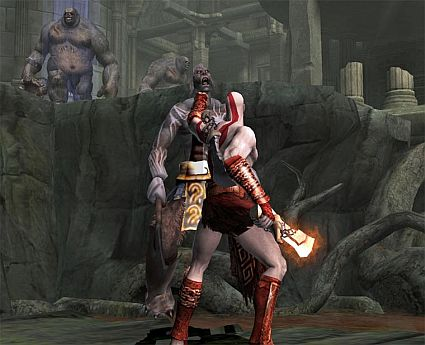
\includegraphics[scale=0.3]{imagens/gow2}
		\end{figure}
\end{frame}

\begin{frame}{História dos Vídeo Games}
\begin{itemize}
	\item Setima Geração(2005 - presente)\pause
	\begin{itemize}
		\item 3D chega aos portáteis no DS e PSP\pause
		\item Blu-Ray e HD-DVD surgem como mídia para jogos\pause
		\item Armazenamento em HD nos Vídeo Games\pause
		\item consoles com jogos online\pause
		\item O corpo se torna um novo controle(wii, ps Move e MS Kinect) e revoluciona Gameplay\pause
		\item Brasil volta ao Mercado de Jogos\pause
		\item Uso de Vídeo Games para computação de alto desempenho(PS3)\pause
		\item 2005 - XBOX 360\pause
		\item 2006 - PS3 e Wii\pause
		\item 2010 - Microsoft Kinect\pause
		\end{itemize}
		\end{itemize}
				\begin{figure}[t]
			    \centering
				    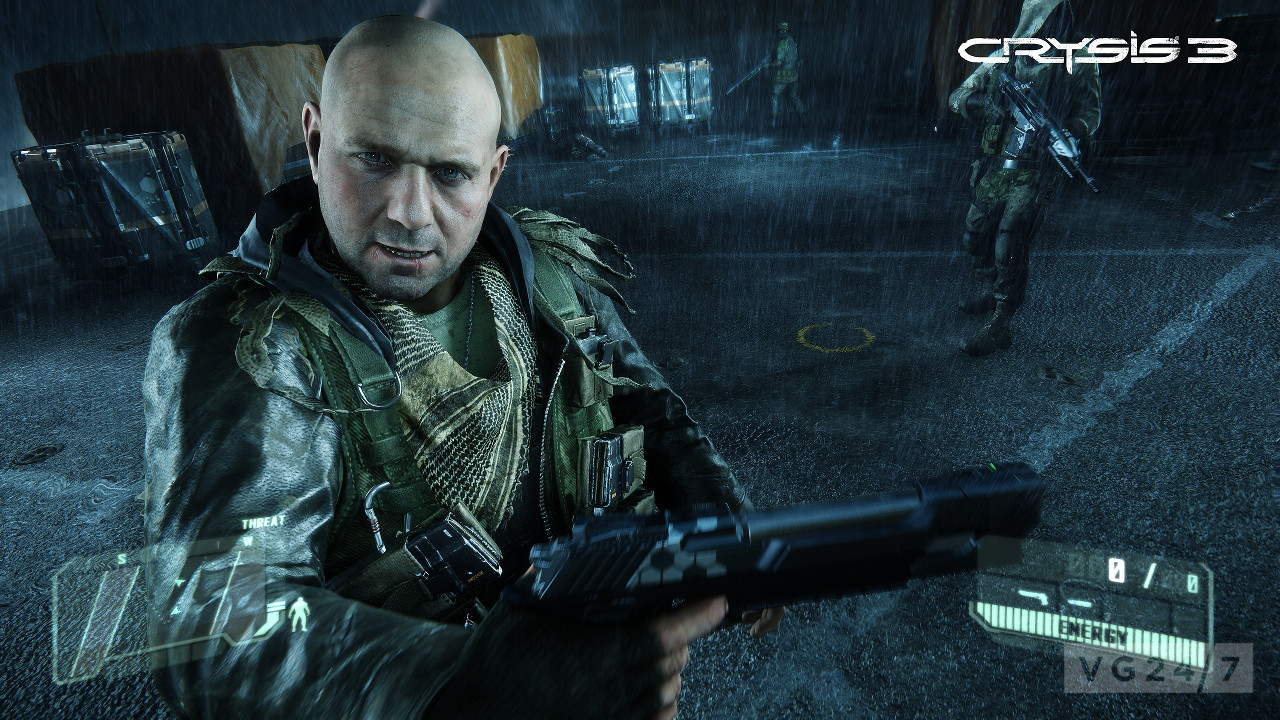
\includegraphics[scale=0.1]{imagens/c3}
				\end{figure}
\end{frame}

\begin{frame}{História dos Vídeo Games}
\begin{itemize}

	\item Oitava Geração(2012 - presente)\pause
	\begin{itemize}
		\item 2012 - WiiU\pause
		\item 2013 - XBOX One e PS4
	\end{itemize}
\end{itemize}
				\begin{figure}[t]
			    \centering
				    
\includegraphics[scale=0.07]{imagens/ryse}
				\end{figure}
\end{frame}
%---
	
\begin{frame}{SNES}
\section{SNES}

\begin{figure}[t]
    \centering
    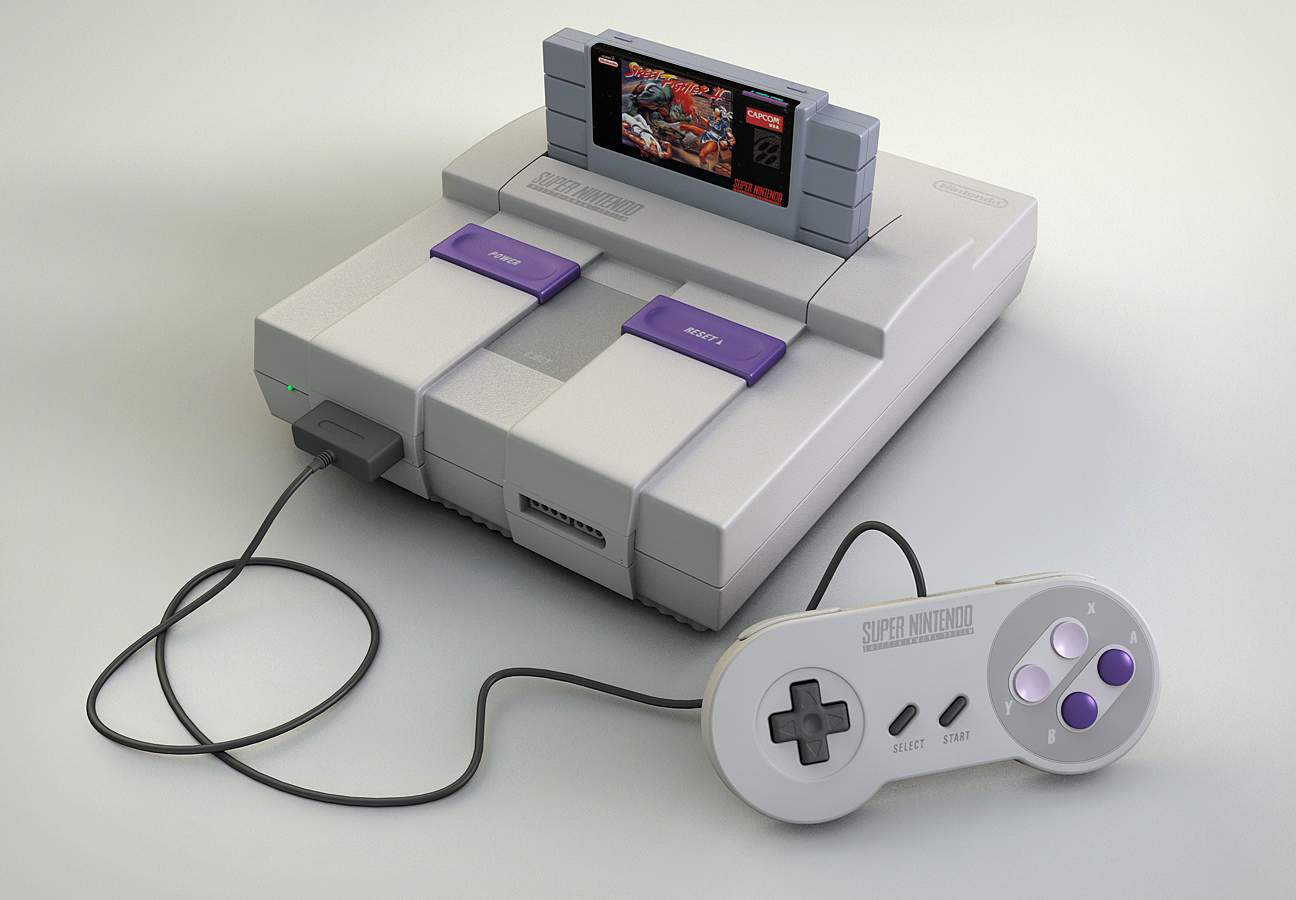
\includegraphics[scale=0.2]{imagens/snes}
\end{figure}
\end{frame}


%------------------------------------------------

\begin{frame}{Especificações Técnicas}
\subsection{Especificações Técnicas}

\begin{itemize}
  \item{Arquitetura 16-bits}
  \item{32768 $(2^{15})$ cores}
  \item{Som com 8 canais de alta qualidade (32kHz - 16 bit Stereo)}
\end{itemize}

\begin{figure}
  \begin{center}
    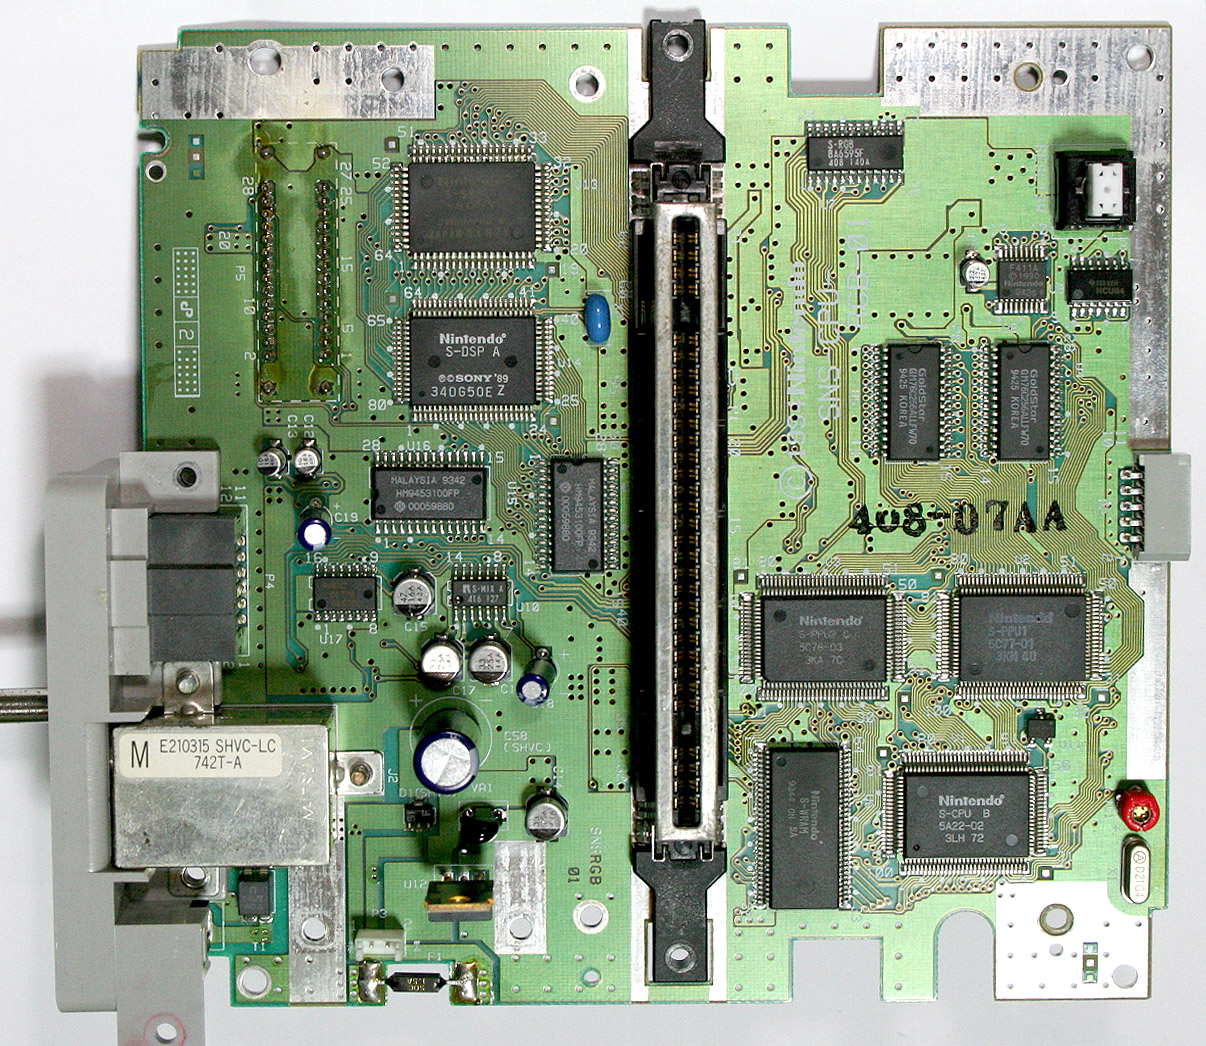
\includegraphics[height=5cm, width=\textwidth, keepaspectratio]{SNES-CPU-RGB01_01.jpg}
    \label{fig:}
    \caption{Placa-Mãe do SNES}
  \end{center}
\end{figure}

\end{frame}

%------------------------------------------------

\begin{frame}{CPU}
\section{A CPU}
  \begin{itemize}
    \item{Chip customizado da Nintendo baseado no microprocessador 65c816}
    \item{Clock 21.47727 MHz (NTSC)/ 21.28137 MHz (PAL) divididos em 6, 8 ou 12.}
    \begin{itemize}
      \item{6:  Acessos gerais}
      \item{8:  Acesso a WRAM}
      \item{12: Acesso aos controles}
    \end{itemize}
    \item{Barramento de dados de 8-bit, controlado por 2 barramentos de endereços:}
    \begin{itemize}
      \item{Bus "A" (24-bit): Acesso geral}
      \item{Bus "B" (8-bit): Suporte aos processadores de áudio e vídeo.}
    \end{itemize}
    \item{Usa DMA (Direct Access Memory) para atingir até 2.68 MB/s de transferência de dados.}
  \end{itemize}
\end{frame}

%------------------------------------------------

\begin{frame}{Vídeo}
\section{O Vídeo}
    \begin{itemize}
      \item{64kB de SRAM}
      \item{544bytes de OAM (Object Attribute Memory) para armazenar sprites}
      \item{256x15 bits de CGRAM (Color Generator RAM) para a paleta de cor}
      \item{Diferentes resoluções PAL/NTSC e Progressivo/Entrelaçado}
      \begin{itemize}
        \item{Progressivo: 256 × 224, 512 × 224, 256 × 239, 512 × 239}
        \item{Entrelaçado: 512 × 448, 512 × 478}
      \end{itemize}
      \item{Pixel Depth: Indexado e direto}
    \end{itemize}
\end{frame}

\begin{frame}{Vídeo}
    \begin{itemize}
      \item{Diferentes modos com resolução, número de camadas e esquema de cores diferentes}
      \begin{itemize}
        \item{Modo 7 suporta rotação e dilatação de camadas usando transformações de matrizes}
      \end{itemize}
    \end{itemize}
  \begin{figure}
  \begin{center}
    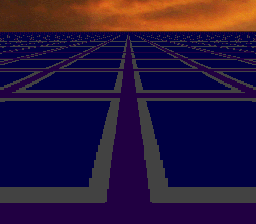
\includegraphics[height=4.5cm, width=\textwidth, keepaspectratio]{Mode_7.png}
    \label{fig:}
    \caption{Modo 7}
  \end{center}
\end{figure}
\end{frame}

%------------------------------------------------

\begin{frame}{Áudio}
\section{O Áudio}
\begin{itemize}
  \item{8-bit Sony SCP700, 16-bit DSP (Processador de Sinal Digital)}
  \item{64kB dse SRAM compartilhada e 64 bytes de Boot ROM}
  \item{Clock: 24.576 MHz}
  \item{Praticamente independente do resto do sistema}
  \item{Comunicação com a CPU é feita apenas via 4 registradores do Bus B}
  \item{Acesso à RAM multiplexado entre o SCP700(1/3) e o DSP(2/3)}
  \item{O SPC700 roda programas carregados pela Boot ROM e aceita instruções e dados da CPU para manipular o DSP e gerar o áudio}
\end{itemize}
\end{frame}

%------------------------------------------------

\begin{frame}{Cartucho}
\section{Cartucho}
\begin{itemize}
	\item Snes pode endereçar 128Mbit, apenas 117Mbit para uso do cartucho\pause
	\item Um cartucho contem em geral 95Mbit de espaço para ROM mais 8Mbit saves\pause
	\item Apesar do espaço, os maiores jogos ocupavam 48Mbit\pause
	\item Os saves são guardados em capacitores, e mantidos à bateria\pause
	\item Máximo de 62 pinos, a um clock de 21,477 MHz
\end{itemize}
\begin{figure}
  \begin{center}
    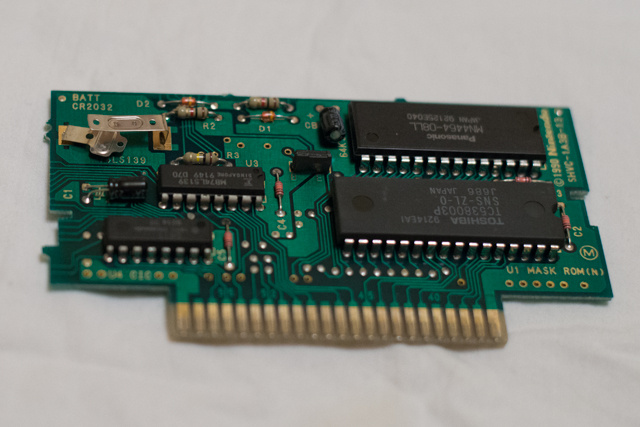
\includegraphics[height=4cm, width=\textwidth, keepaspectratio]{imagens/cartucho}
    \label{fig:}
  \end{center}
\end{figure}
\end{frame}

\begin{frame}{Enhancement Chips}
\subsection{Enhancement Chips}
\begin{itemize}
  \item{Plano: Evitar que a CPU fosse complexa e cara e ficasse obsoleta em pouco tempo}
  \item{Design: Co-processadores podiam ser adicionados no cartucho, e a interface era feita utilizando mais pinos}
\end{itemize}
\begin{figure}
  \begin{center}
    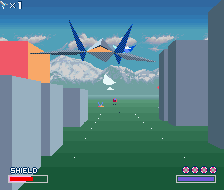
\includegraphics[height=4cm, width=\textwidth, keepaspectratio]{SNES_Star_Fox.png}
    \label{fig:}
    \caption{Star Fox utilizando o chip Super FX}
  \end{center}
\end{figure}
\end{frame}

\begin{frame}{CIC e Pirataria}
\section{CIC e Pirataria}
\begin{itemize}
\item Composto por um microcontrolador no console que checa ao cartucho inserido para autenticação.
\item Enquanto o cartucho não responder ou responder errado então o CIC reseta a CPU a cada ciclo.
\item O reinício constante da CPU impedia o console de ser inicializado.
\end{itemize}
\begin{figure}
  \begin{center}
    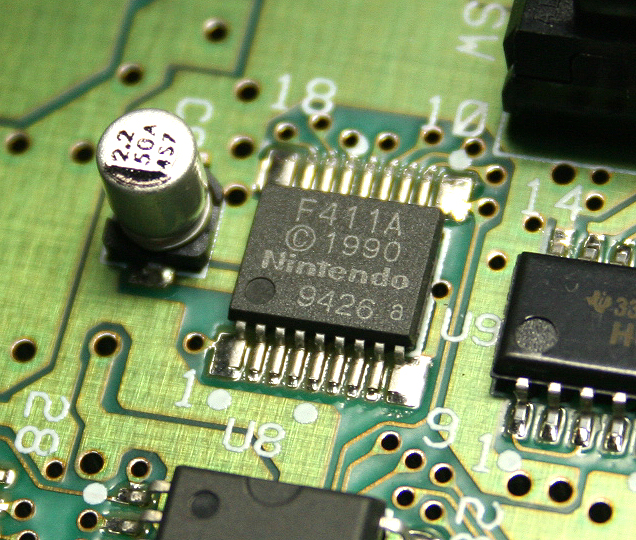
\includegraphics[height=4.7cm, width=\textwidth, keepaspectratio]{imagens/cic}
    \label{fig:}
  \end{center}
\end{figure}
\end{frame}
%------------------------------------------------

\begin{frame}{Mão na massa}
\section{Mão na massa}
\begin{itemize}
  \item{Como era feita a programação?}
  \item{Código simples que inicializa o console e muda a cor de fundo}
  \item{Código da trilha sonora do Top Gear}
  \item{Código mais complexo - Jogo da Velha}
\end{itemize}
\end{frame}

%------------------------------------------------

\begin{frame}{Conclusões}
\section{Conclusões}
\begin{itemize}
  \item{O SNES é muito mais complexo do que parece}
  \item{A documentação é toda não-oficial e só muito recentemente (últimos 5 anos) vem sendo organizada}
  \item{É uma pena que a documentação oficial, desde os datasheets dos componentes até o código fonte em ASM dos jogos, nunca foi publicada.}
  \item{O estudo do console deu uma ótima visão de como todos os componentes funcionam em conjunto}
  \item{O estudo dos códigos em Assembly mostrou vários aspectos práticos interessantes, como a ausência de frameworks e até aspectos bastante técnicos, como o V-Blank}
\end{itemize}

\end{frame}
%------------------------------------------------

\begin{frame}{Referências}
\begin{itemize}
\item História dos Vídeo Games:
\begin{itemize}	
\item http://en.wikipedia.org/wiki/History\_of\_video\_games
\end{itemize}
\item Hardware geral:
\begin{itemize}	
\item 	http://www.caitsith2.com/snes/
\item 	http://digitalfantasy.angelfire.com/snes-hardware-specifications.html
\item 	http://en.wikipedia.org/wiki/Super\_Nintendo\_Entertainment\\\_System\_technical\_specifications
\item 	http://de.academic.ru/dic.nsf/dewiki/1219157
\item 	http://pikensoft.com/old/docs/SNES\_chip\_labels.txt
\item 	http://nocash.emubase.de/fullsnes.txt
\end{itemize}
\end{itemize}
\end{frame}

\begin{frame}{Referências}
\begin{itemize}
\item Áudio:
\begin{itemize}	
\item 	http://en.wikipedia.org/wiki/Nintendo\_S-SMP
\item 	http://snesmusic.org/v2
\item 	http://snesmusic.org/files/spc700.html
\item 	http://web.archive.org/web/20090106230547/http://www.a\\lpha-ii.com/snesmusic/files/spc700\_apu\_manual.txt
\end{itemize}
\item Processador:
\begin{itemize}	
\item 	http://en.wikipedia.org/wiki/WDC\_65816/65802
\item 		http://westerndesigncenter.com/wdc/docume\\ntation/w65c816s.pdf
\item 	http://en.wikibooks.org/wiki/6502\_Assembly
\end{itemize}
\item Programação:
\begin{itemize}	
\item 	http://en.wikibooks.org/wiki/Super\_NES\_Programming
\item 	http://wiki.superfamicom.org/snes/show/HomePage
\end{itemize}
\end{itemize}
\end{frame}

\begin{frame}{Referências}
\begin{itemize}
\item ROM Hacking:
\begin{itemize}	
\item 	http://www.romhacking.net
\item 	http://www.romhacking.net/start/
\end{itemize}
\item Controle:
\begin{itemize}	
\item www.gamesx.com/controldata/snesdat.htm
\end{itemize}
\item CIC:
\begin{itemize}	
\item en.wikipedia.org/wiki/CIC\_(Nintendo)
\end{itemize}
\item Cartucho:
\begin{itemize}
\item http://motherboard.vice.com/blog/pictures-how-to-replace-an-snes-cartridge-save-game-battery
\item http://www.caitsith2.com/snes/flashcart/cart-chip-pinouts.html
\end{itemize}
\end{itemize}

\end{frame}

\begin{frame}{Dúvidas}
	\begin{itemize}
	\item Dúvidas?
	\end{itemize}
\end{frame}

%------------------------------------------------

%----------------------------------------------------------------------------------------

\end{document}


\section{Introdução}  % add these to see outline in slides

\section*{Introdução}

\subsection*{\underline{Escolha do software}:}

No início da disciplina, resolvemos escolher entre um dos projetos
recomendados pelo professor Daniel, assim como fizeram a maioria dos outros
grupos. Em particular demos preferência àqueles documentados no
\href{http://flosscoach.com}{FLOSS Coach},como indicado pelo professor.

\begin{wrapfigure}{l}{0.3\textwidth} % Inline image example
\begin{center}

\includegraphics[width=0.28\textwidth]{src/empathy_logo.jpg}
\caption*{Empathy}
\end{center}
\end{wrapfigure}

Dentre os projetos da lista, levantamos os pontos positivos e negativos
em trabalhar com cada um deles e também ponderamos nossas preferências
pessoais. Finalmente, chegamos a conclusão de trabalhar com o Empathy, um
\emph{messenger} que funciona com diversos protocolos e que faz parte do projeto
Gnome. Consideramos pontos positivos a familiaridade com a linguagem (C++), o
tamanho médio do projeto, a existência de bugs apropriados à nossa capacidade e
o interesse de utilização de um software mensageiro.

Durante o semestre, depois
de muito tempo gasto tentando compilar o código-fonte, perdemos um pouco a
motivação e levantamos a possibilidade de mudar de projeto.
Ao mesmo tempo, tivemos
contato com o projeto Pixelated durante a CryptoRave e decidimos seguir com ele
devido à sua declarada abertura à comunidade, nosso interesse no objetivo de
disseminação de comunicação criptografada e também nas ferramentas utilizadas.

O Pixelated é um projeto que se compromete a servir emails de forma segura e
distribuída com foco na usabilidade do usuário, com a
proposta de substituir os clientes de email atuais por um padrão criptografado.

\subsection*{\underline{Início da jornada}:}
Começamos então a compilar o Empathy e tivemos muitos problemas desde o início.
Iniciamos o processo de compilação em 3 distribuições diferentes (ArchLinux,
Debian e Ubuntu) e tivemos muita dificuldade em todas elas.

Como o Empathy faz parte do projeto Gnome, ele possui várias dependências:
\begin{lstlisting}[language=bash]
	gnome-common, gettext, libglib2.0-dev, gtk-doc-tools, libxml2-dev, libtelepathy-glib-dev, libmissioncontrol-client-dev, libtelepathy-farsight-dev, libx11-dev, libgtk2.0-dev, libice-dev{a}, libcanberra-gtk-dev, libgstreamer-plugins-base0.10-dev, libebook1.2-dev, libnotify-dev, libunique-dev, libgnome-keyring-dev, libtelepathy-logger-dev, libwebkitgtk-3.0-dev, libgnutls-dev, libfolks-telepathy-dev, libcanberra-gtk3-dev, libgcr-3-dev, gsettings-desktop-schemas-dev
\end{lstlisting}
Na primeira tentativa de compilação faltaram as seguintes dependências:
\begin{lstlisting}[language=bash]
  libyelp-dev yelp-tools -> itstool{a} libxslt1-dev{a} libyelp-dev yelp-tools zip{a}
  libsecret-1
\end{lstlisting}
    E essas outras estavam em versões antigas:
\begin{lstlisting}[language=bash]
  {glib-2.0,gio-2.0} >= 2.33.3 -> 2.32.4 encontrado
  telepathy-glib >= 0.22.0 -> 0.18.2 encontrado
  gtk+-3.0 >= 3.5.1 -> 3.4.2 encontrado
  	glib-2.33.3 -> libffi-dev (3.0.10-3)
  	gtk+-3.6.0 -> glib-2.0 >= 2.33.1 -> 2.32.4 encontrado
               -> atk >= 2.5.3 -> 2.4.0 encontrado
\end{lstlisting}
Na segunda tentativa o \texttt{configure} passou nos testes para gerar o
primeiro binário mas falhou no segundo:
Faltaram as seguintes dependências:
\begin{lstlisting}[language=bash]
gee-0.8
libpulse-mainloop-glib
libpulse
\end{lstlisting}
E essas outras estavam em versões antigas:
\begin{lstlisting}[language=bash]
folks >= 0.9.5 -> 0.6.9 encontrado
folks-telepathy >= 0.9.5 -> encontrado 0.6.9
glib-2.0 >= 2.37.6' -> 2.33.3 encontrado
gio-2.0 >= 2.37.6' -> 2.33.3 encontrado
gio-unix-2.0 >= 2.37.6 -> 2.33.3 encontrado
telepathy-glib >= 0.23.2 -> 0.22.0 encontrado
telepathy-logger-0.2 >= 0.8.0 -> 0.4.0 encontrado
gtk+-3.0 >= 3.9.4 -> 3.6.0 encontrado
webkitgtk-3.0 >= 1.9.1 -> 1.8.1 encontrado
\end{lstlisting}

Além das mesmas complicações, agora tivemos que compilar o webkitgtk-3.0.
Essa dependência causou muito desgaste. Em particular, neste ponto, descobrimos
que deveríamos ter instalado uma biblioteca chamada VALA antes de iniciar todo o
processo de compilação.
Compilamos o VALA necessário, recompilamos todas as dependências, e tentamos
compilar o webkitgtk-3.0. Durante a compilação, ocorreu um erro dizendo que os
arquivos VALA estão inconsistentes (redeclaração de classe). Nesse ponto ficamos
bastante decepcionados com o projeto.

Além disso, existe uma iniciativa para ajudar iniciantes que queiram começar
a colaborar com projetos do gnome. Uma das ações dessa iniciativa é a de marcar
bugs adequados para iniciantes com a tag gnome-love. Quando fomos pesquisar bugs
do Empathy no bugtracker do projeto, procuramos pela tag gnome-love e, para
nossa surpresa e desapontamento, encontramos apenas três bugs com essa tag.

Esse conjunto de motivos nos levou a abandonar o projeto Empathy e a procurar
por um projeto mais amigável para desenvolvedores iniciantes.


\section{Desenvolvimento}
\begin{frame}
%\note[item]<100>{As músicas automáticas foram gravadas com um piano MIDI}
%\note[item]<100>{As músicas anotadas foram anotadas manulmente, no nível de nota no rachmaninoff e pulso para as sinfonias}
%\note[item]<100>{7 Performances adicionais foram coletadas sem anotação, apenas para serem processadas de forma automática. Com exceção das que já tem 22 (7 foram escolhidas aleatoriamente dentre elas, sem repetir o performer)}
%\note[item]<100>{dizer que existem duas musicas orquestrais, dificuldade maior}
%\note[item]<100>{dizer que foi obtido mais de uma gravação da mesma musica}
  \frametitle{Descrição dos dados}
  \pause
  \begin{center}
    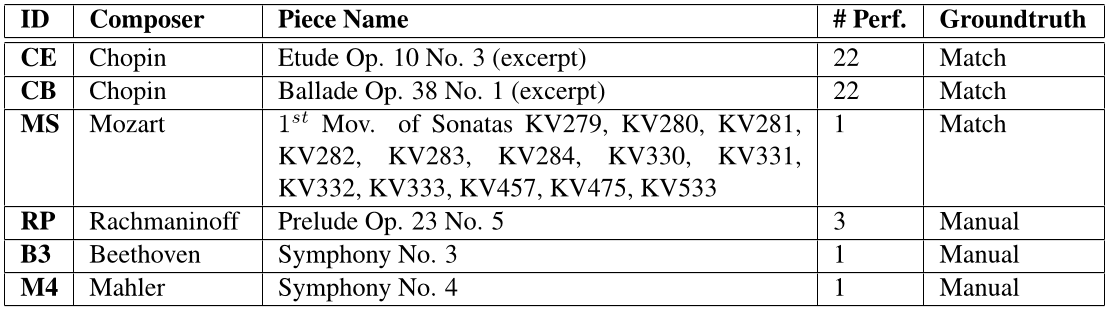
\includegraphics[width=\textwidth]{src/img/1-Table1-1.png}
  \end{center}
\end{frame}

\begin{frame}
  \frametitle{Rastreamento padrão baseado em representação simbólica musical}
  Abordagem baseada no algoritmo \emph{Dynamic Time Warping (DTW)} com algumas extensões:\pause
%\note[item]<100>{  que possibilitam a aplicação em rastreamento online. [artigo 10]}
  \begin{itemize}
    \item O caminho é computado de maneira incremental\\\pause
    \item A complexidade é reduzida para ser linear no tamanho da entrada\pause
    \item Utiliza a estratégia \emph{backward-forward}
%\note[item]<100>{reconsidera decisoes passadas, aumenta robustez [artigo 4]}
%\note[item]<100>{ aumenta a habilidade de o algoritmo lidar com diferencas no Andamento [artigo 3] }
  \end{itemize}
\end{frame}

\begin{frame}
  \frametitle{\emph{Dynamic Time Warping (DTW)}}
  \begin{center}
    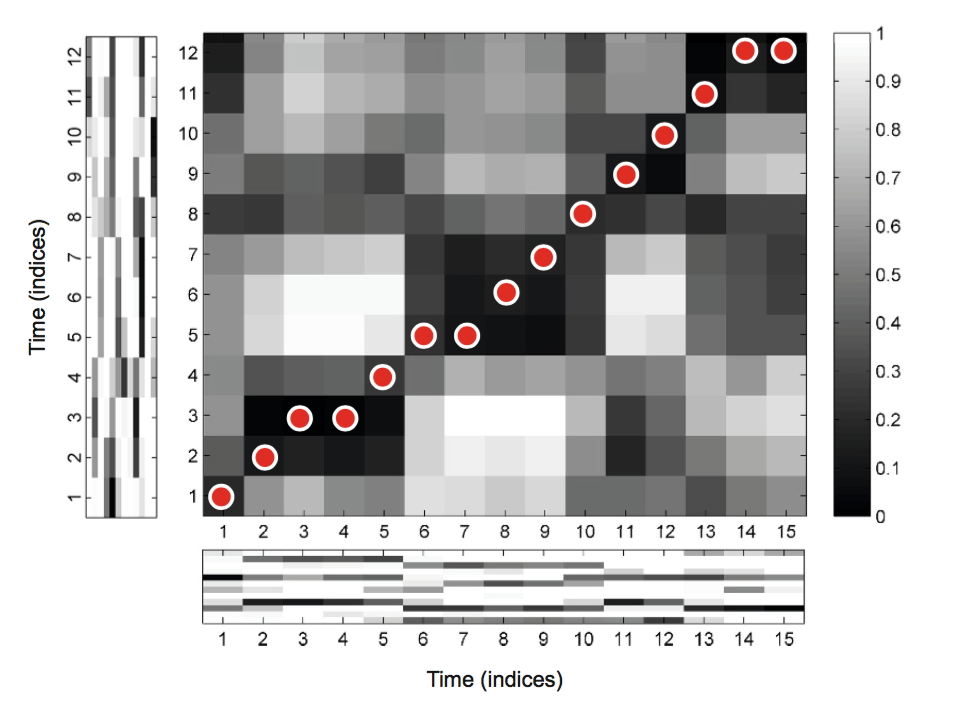
\includegraphics[width=0.7\textwidth]{src/img/dtw.png}
  \end{center}
\end{frame}

\begin{frame}
  \frametitle{Características}
  \begin{center}
    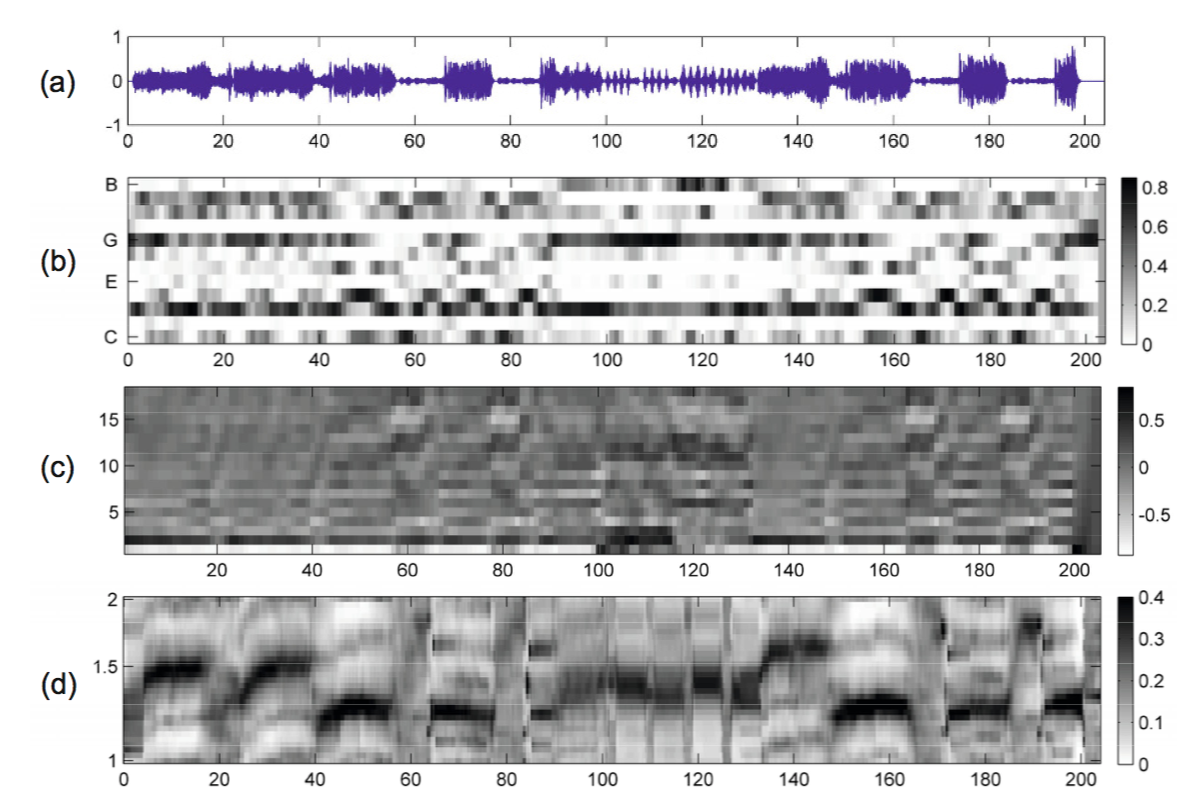
\includegraphics[width=0.7\textwidth]{src/img/caracteristicas.png}
  \end{center}
\end{frame}

\begin{frame}
  \frametitle{Cromagrama}
  \begin{center}
    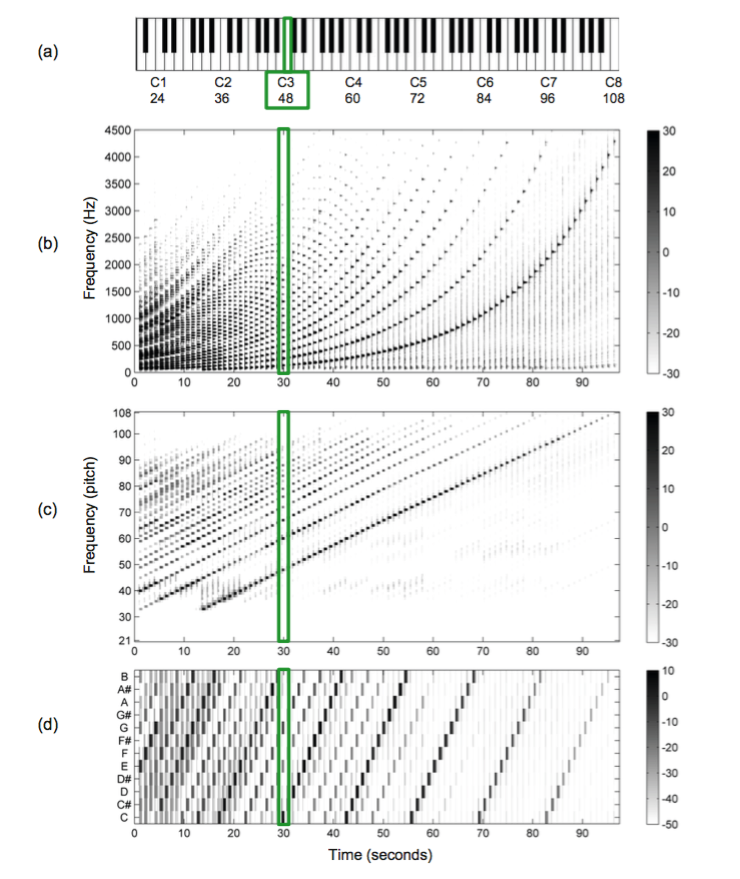
\includegraphics[width=0.45\textwidth]{src/img/cromagrama.png}
  \end{center}
\end{frame}

\begin{frame}
  \frametitle{Rastreamento padrão baseado em representação simbólica musical}
  %\note[item]<100>{ Para ser possível o tracking é necessário...}
  Precisamos de uma representação da partitura\pause
  \begin{itemize}
    \item Síntese MIDI -> áudio\\\pause
    \item Alinhamento áudio-áudio, agora com a informação temporal de cada nota\pause
  \end{itemize}
  Nesse artigo, é usado uma mistura de características cromáticas e de início de nota \emph{(semi-tone onset)} e o algoritmo explicado anteriormente
\end{frame}

\begin{frame}
  \frametitle{Resultados utilizando o rastreamento padrão}
  \begin{center}
    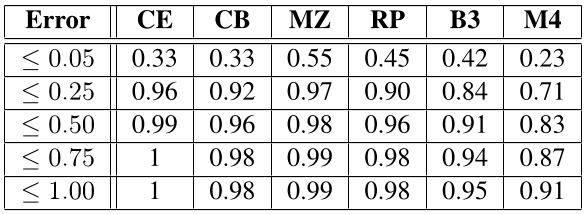
\includegraphics[width=0.8\textwidth]{src/img/1-Table2-1.png}
  \end{center}
  \pause
  \begin{itemize}
    \item Funciona bem para peças em piano\\\pause
    \item Não funciona bem para peças orquestrais
    %\note[item]<100>{É fácil sintetizar piano mas é muito mais complexo para orquestras}
  \end{itemize}
\end{frame}

\begin{frame}
  \frametitle{Rastreamento utilizando uma performance como referência}
  O rastreamento padrão funciona bem mas ganhamos algumas vantagens ao utilizar uma performance real como referência:\pause
  \begin{itemize}
    \item Melhor qualidade
    \item Características mais próximas da performance ao vivo que queremos rastrear
    \item Maior similaridade sonora, principalmente em peças orquestradas
    \item Informações detalhadas de andamento, dinâmica e articulação
  \end{itemize}
\end{frame}

\begin{frame}
  \frametitle{Rastreamento utilizando uma performance como referência}
  Porém, temos uma grande desvantagem:\pause
  \begin{itemize}
    \item A informação temporal das notas é inexistente\pause
  \end{itemize}
  Assim, precisaremos calcular esta informação para seguir essa abordagem. \pause Nesse artigo, isso será feito de forma automática
\end{frame}

\againframe<1>{figura1}

\begin{frame}
  \frametitle{Alinhamento off-line}
  \begin{itemize}
    \item Espera-se que o aumento na qualidade das características supere o erro introduzido por esta etapa\pause
    \item Aqui, usamos o algoritmo já citado, com a única diferença de que, no final, computamos o caminho contrário, como se faz no DTW padrão.
    %\note[item]<100>{ É claro que podemos usar qualquer algoritmo de alinhamento}
  \end{itemize}
  Assim, temos resultados melhores que o caso online.
\end{frame}

\begin{frame}
  \frametitle{Comparação dos resultados}

  \begin{figure}[!tbp]
    \centering
    \begin{minipage}[b]{0.45\textwidth}
      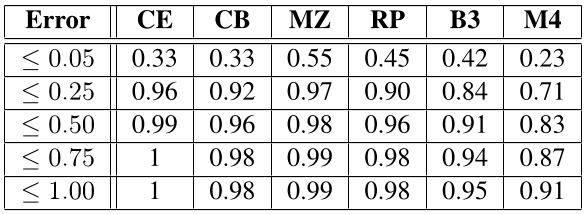
\includegraphics[width=\textwidth]{src/img/1-Table2-1.png}
      \caption*{Rastreamento padrão}
    \end{minipage}
    \hfill
    \begin{minipage}[b]{0.45\textwidth}
      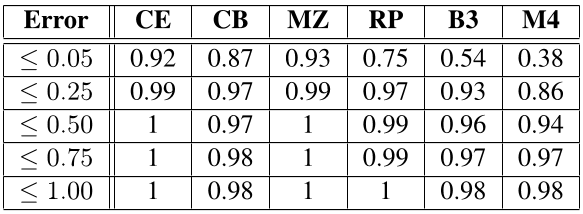
\includegraphics[width=\textwidth]{src/img/1-Table3-1.png}
      \caption*{Alinhamento off-line}
    \end{minipage}
  \end{figure}
\end{frame}

\begin{frame}
  \frametitle{Rastreamento baseado em uma performance alinhada}
  Agora, utilizando a performance já alinhada, utilizamos o mesmo algoritmo de rastreamento para as outras performances.
  Estes são os resultados:
  \begin{figure}[!ht]
    \centering
    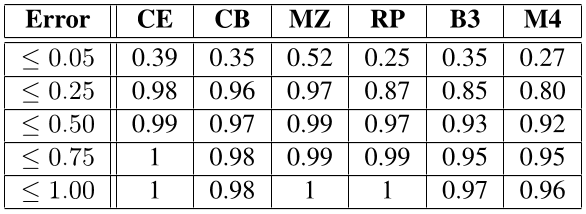
\includegraphics[width=0.7\textwidth]{src/img/3-Table4-1.png}
    \caption*{Rastreamento on-line baseado em uma performance alinhada off-line}
  \end{figure}
\end{frame}

\begin{frame}
  \frametitle{Rastreamento baseado em uma performance alinhada}
  \begin{itemize}
    \item Melhoria nas peças orquestradas\pause
    \item Resultados se mostraram instáveis - algumas performances são mais similares entre si do que com a usada como referência \pause %Infelizmente
    \item Resultados mostraram que algumas partes da peça tiveram erros em muitos rastreamentos \pause %A peça é difícil mesmo
    \item Utilizando diferentes performances como referência, alguns erros só apareciam em uma ou duas delas \pause
  \end{itemize}
  Isto levou à ideia de combinar o alinhamento de várias performances para diminuir estes erros.
\end{frame}

\begin{frame}[label=figura2]
  \frametitle{Rastreamento baseado em várias performances alinhadas}
  \begin{figure}[!ht]
    \centering
    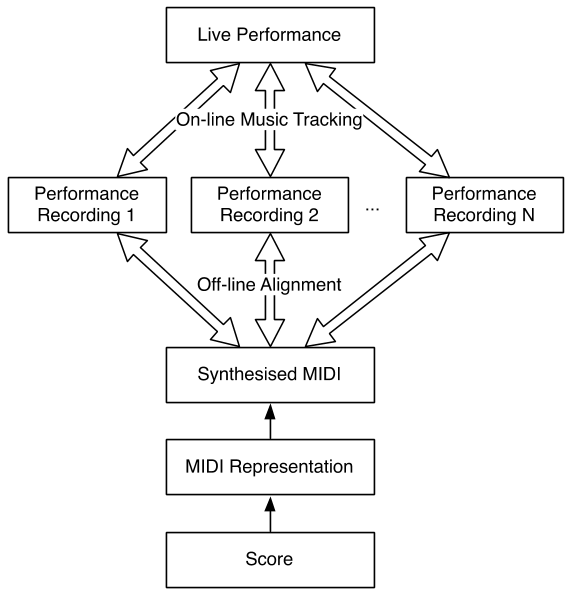
\includegraphics[height=0.7\textheight]{src/img/2-Figure2-1.png}
    \caption*{Rastreamento multi-agente baseado em várias performances alinhadas off-line}
  \end{figure}
\end{frame}

\begin{frame}
  \frametitle{Rastreamento baseado em múltiplas performances}
  \begin{itemize}
    \item Várias anotações alinhadas são usadas em paralelo no rastreamento\pause
    \item Utilizamos a mediana \pause %Explicar o porquê
    \item Mais estabilidade em aplicações práticas \pause
    \item Foram utilizadas 7 performances
%\note[item]<100>{explicar tradeoff robustez x tempo de computação}
  \end{itemize}
\end{frame}


\section{Resultados}
\begin{frame}
  \frametitle{Comparação dos resultados}

  \begin{figure}[!tbp]
    \centering
    \begin{minipage}[b]{0.45\textwidth}
      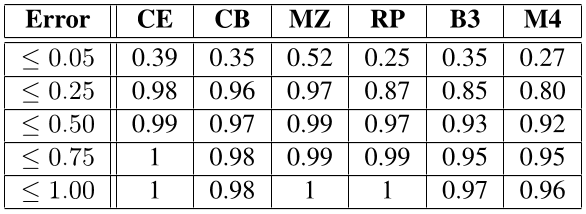
\includegraphics[width=\textwidth]{src/img/3-Table4-1.png}
      \caption*{Apenas uma performance como referência}
    \end{minipage}
    \hfill
    \begin{minipage}[b]{0.45\textwidth}
      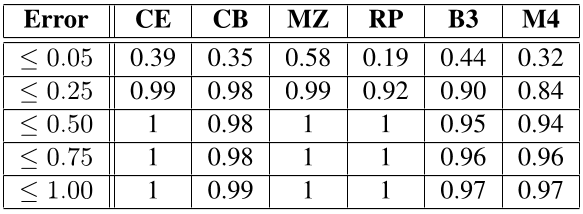
\includegraphics[width=\textwidth]{src/img/3-Table5-1.png}
      \caption*{Múltiplas performances como referência}
    \end{minipage}
  \end{figure}
\end{frame}

\begin{frame}
  \frametitle{Comparação de todos os resultados}
  \begin{center}
    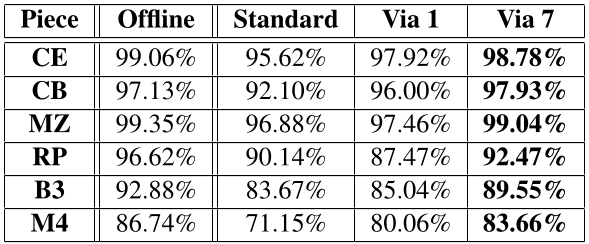
\includegraphics[width=0.8\textwidth]{src/img/4-Table6-1.png}
  \end{center}
  \begin{itemize}
    \item Melhores resultados do que o alinhamento off-line\pause
    \item Erros introduzidos no alinhamento off-line impactaram menos do que a melhora de qualidade no método
  \end{itemize}
\end{frame}


\section{Cenário real}
\begin{frame}
  \frametitle{Projeto PHENICX}
  \begin{itemize}
    \item Projeto que visa melhorar a experiência da música clássica\pause
    \item Videodock criou a interface de usuário e as visualizações \pause
  \end{itemize}
  O grande evento: \pause
  \begin{itemize}
    \item Dia 7 de Fevereiro de 2015
    \item Concertgebouw - Amsterdam
    \item The Royal Concertgebouw Orchestra, conduzida por Semyon Bychkov
    \item Alpensinfonie - Richard Strauss
    \item Nenhum acesso à representação simbólica - Anotação feita à mão (downbeat) para uma performance
    \item Outras 6 performances alinhadas com essa primeira
  \end{itemize}
\end{frame}


\section{Conclusão}
\section*{Conclusões}

\subsection*{\underline{Ser voluntário é fácil?}:}
Depende do projeto! No Empathy, não tivemos ninguém para ajudar e acabamos
deixando-o sem nem tê-lo compilado.

Já no Pixelated, apesar de a documentação ser de um certo modo escassa, a
comunidade e os desenvolvedores foram bem receptivos a novos colaboradores,
constantemente disponíveis no IRC e no GitHub. Como a ThoughtWorks tem um plano
de fomentar a auto-sustentação da comunidade, a barreira de entrada nesse caso
foi mínima.

Uma outra questão importante é o tempo disponível. O voluntariado é lindo na
teoria mas é muito difícil na prática. Muitas vezes gostaríamos de estar
trabalhando no projeto mas todos os integrantes do grupo fazem estágio além de
estudar para outras disciplinas do IME. Sendo assim, achamos que a
contribuição de profissionais (como acontece no caso do Pixelated) é muito
importante para o sucesso de um projeto de Software Livre.

\subsection*{\underline{Formação}:}

A partir do que aprendemos na disciplina, concluímos que contribuir para um
projeto de Software Livre é um excelente acréscimo para a formaçao de qualquer
aluno de computação porque são necessárias diversas habilidades para tal, desde
habilidades técnicas até habilidades pessoais de comunicação que, infelizmente,
são constantemente negligenciadas em nossa formação.

Entre as habilidades técnicas desenvolvidas, destaca-se a habilidade de ler
código escrito por outras pessoas, a habilidade de escrever código de qualidade
que seja legível por outros, a utilização de softwares de controle de versão e a
habilidade de aprender novas tecnologias e padrões de projeto. Entre as
habilidades não-técnicas destacamos a comunicação, seja online pelo IRC, seja ao
vivo em conferências de Software e o engajamento em uma comunidade onde todas as
partes têm experiências e conhecimentos diferentes e trabalham para um objetivo
comum. Nosso trabalho com o Pixelated tocou em todos desses pontos.

A experiência de trabalhar em um projeto de software livre desenvolve uma
miríade de habilidades e, portanto, é um grande diferencial na formação do
nosso curso.


\subsection*{\underline{Falhas na comunidade}:}

A documentação é bastante escassa, não existe uma página que concentre informaçoes importantes, dedicada a guiar novos desenvolvedores. Isso certamente fez falta em alguns momentos, e tivemos que gastar tempo tirando dúvidas diretamente com os desenvolvedores, via IRC.
Sugerimos que seja criada ao menos uma página com as informações básicas, por exemplo "quais passos seguir antes de enviar um pull request", ou em linhas gerais "como funciona a estrutura da parte javascript do projeto".
Acreditamos que essas páginas ainda não existam pois o projeto é novo, e ainda é fácil contactar os desenvolvedores diretamente. Devemos confessar que nós, como desenvolvedores, entendemos como é dificil lidar com documentaçao em qualquer projeto, mas cedo ou tarde eles provavelmente sentirão essa necessidade e resolverão o problema.

\subsection*{\underline{Pré-requisitos}:}

Para acompanhar as aulas não é necessário muito conhecimento prévio, até porque as palestras apresentadas pelos alunos são introdutórias.
Para contribuir com algum projeto de software livre isso já muda. Porém, é muito difícil responder essa questão, pois o conhecimento necessário é bastante relativo. Depende em qual projeto o aluno vai trabalhar.
Para poder contribuir eficientemente com um projeto de software livre muitas habilidades são necessárias, não só técnicas, como também de comunicação. Quanto mais experiência com diversas linguagens e tecnologias, melhor. Quanto mais experiência com o ecossistema de software livre, melhor. Quanto mais experiência com desenvolvimento de software em equipe, melhor. O difícil é dizer o quanto é necessário de cada um.
É essencial ter bastante vontade de aprender ao cursar essa disciplina, é quase certo que, ao começar a colaborar com um projeto, será necessário aprender algumas tecnologias novas, aprender a se comunicar com aquela comunidade em particular e também aprender como o software funciona a fundo, lendo seu código.
    Vale destacar que conhecer bem o sistema operacional no qual se trabalha ajuda e muito o desenvolvimento do projeto. No caso do empathy por exemplo, pudemos avançar até tal ponto pois tínhamos um conhecimento abrangente do sistema, como ligar bibliotecas, o que significa cada linha de comando que executávamos e como consertar em caso de alguma inconsistência. Para se ter idéia, todas as bibliotecas (dependências) que instalamos, mesmo sendo em uma máquina virtual somente para o projeto da disciplina, foram instaladas em um diretório específico para que tivéssemos certeza de que tudo estava sob controle e que as correções ou features novas pudessem ser lançadas sem problemas. Para isso, foi imprescindível ter um bom conhecimento das ferramentas make, configure e pkg-config, de variáveis de ambiente como $LD_LIBRARY_PATH$, PATH e $PKG_CONFIG_PATH$, e de como funciona o ambiente do terminal (env).
Acreditamos que um aluno que fez apenas as disciplinas básicas pode sim fazer a disciplina, contanto que tenha bastante vontade de aprender, mas provavelmente um aluno mais avançado vai conseguir aproveitá-la melhor.


\subsection*{\underline{Tempo gasto}:}

Por fim estimamos o tempo gasto por cada integrante para as várias tarefas do
curso. Esperamos que esse tempo possa servir como referência para uma relação
entre o tempo de trabalho dos diferentes tipos de tarefas realizadas durante o
curso.

Alessandro:
\begin{center}
    \begin{tabular}{ | l | c | p{7cm} |}
    \hline
    Tarefa & Tempo (h) & Detalhes \\ \hline
    Empathy & 10 & Compilando e tentando entender o que deu errado. \\ \hline
    Pixelated & 20 & Bastante tempo lendo sobre criptografia e os protocolos implementados + $\sim$8h compilando e testando o código. \\ \hline
    PT1 & 5 &  \\ \hline
    PNT & 25 & Me empolguei bastante com o tema. \\ \hline
    PT2 & 5 & Mais algumas horas de pesquisas que eu fiz antes da preparação da palestra. \\ \hline
    Relatório & 15 &  \\ \hline
    Aulas & & Presença Obrigatória! \\ \hline
    \end{tabular}
\end{center}

Caio:
\begin{center}
    \begin{tabular}{ | l | c | p{7cm} |}
    \hline
    Tarefa & Tempo (h) & Detalhes \\ \hline
    Empathy & 16 x 4 & Quatro dias inteiros resolvendo erros de compilação: lendo erros e dependências, compilando e ligando tudo. \\ \hline
    Pixelated & 8 x 3 &  \\ \hline
    PT1 & 4 &  \\ \hline
    PNT & 12 &  \\ \hline
    PT2 & 2 &  \\ \hline
    Relatório & 15 &  \\ \hline
    Aulas & & Presença Obrigatória! \\ \hline
    \end{tabular}
\end{center}

Leonardo:
\begin{center}
    \begin{tabular}{ | l | c | p{7cm} |}
    \hline
    Tarefa & Tempo (h) & Detalhes \\ \hline
    Empathy & 8 & $\sim$4h tentando compilar o Empathy no Arch Linux + $\sim$4h pesquisando o bug tracker. \\ \hline
    Pixelated & 12 x 3 & $\sim$4h para executá-lo + $\sim$8h trabalhando na feature a ser implementada + Pull Request. \\ \hline
    PT1 & $\sim$10h & Em média. \\ \hline
    PNT & $\sim$10h & Em média. \\ \hline
    PT2 & $\sim$10h & Em média. \\ \hline
    Relatório & 15 &  \\ \hline
    Aulas & & Presença Obrigatória! \\ \hline
    \end{tabular}
\end{center}


\end{document}
